% Options for packages loaded elsewhere
\PassOptionsToPackage{unicode}{hyperref}
\PassOptionsToPackage{hyphens}{url}
%
\documentclass[
]{article}
\usepackage{lmodern}
\usepackage{amssymb,amsmath}
\usepackage{ifxetex,ifluatex}
\ifnum 0\ifxetex 1\fi\ifluatex 1\fi=0 % if pdftex
  \usepackage[T1]{fontenc}
  \usepackage[utf8]{inputenc}
  \usepackage{textcomp} % provide euro and other symbols
\else % if luatex or xetex
  \usepackage{unicode-math}
  \defaultfontfeatures{Scale=MatchLowercase}
  \defaultfontfeatures[\rmfamily]{Ligatures=TeX,Scale=1}
\fi
% Use upquote if available, for straight quotes in verbatim environments
\IfFileExists{upquote.sty}{\usepackage{upquote}}{}
\IfFileExists{microtype.sty}{% use microtype if available
  \usepackage[]{microtype}
  \UseMicrotypeSet[protrusion]{basicmath} % disable protrusion for tt fonts
}{}
\makeatletter
\@ifundefined{KOMAClassName}{% if non-KOMA class
  \IfFileExists{parskip.sty}{%
    \usepackage{parskip}
  }{% else
    \setlength{\parindent}{0pt}
    \setlength{\parskip}{6pt plus 2pt minus 1pt}}
}{% if KOMA class
  \KOMAoptions{parskip=half}}
\makeatother
\usepackage{xcolor}
\IfFileExists{xurl.sty}{\usepackage{xurl}}{} % add URL line breaks if available
\IfFileExists{bookmark.sty}{\usepackage{bookmark}}{\usepackage{hyperref}}
\hypersetup{
  pdftitle={Análise dataset sobre COVID19 Brasil},
  pdfauthor={Arnaldo Cavalcanti Portfolio},
  hidelinks,
  pdfcreator={LaTeX via pandoc}}
\urlstyle{same} % disable monospaced font for URLs
\usepackage[margin=1in]{geometry}
\usepackage{color}
\usepackage{fancyvrb}
\newcommand{\VerbBar}{|}
\newcommand{\VERB}{\Verb[commandchars=\\\{\}]}
\DefineVerbatimEnvironment{Highlighting}{Verbatim}{commandchars=\\\{\}}
% Add ',fontsize=\small' for more characters per line
\usepackage{framed}
\definecolor{shadecolor}{RGB}{248,248,248}
\newenvironment{Shaded}{\begin{snugshade}}{\end{snugshade}}
\newcommand{\AlertTok}[1]{\textcolor[rgb]{0.94,0.16,0.16}{#1}}
\newcommand{\AnnotationTok}[1]{\textcolor[rgb]{0.56,0.35,0.01}{\textbf{\textit{#1}}}}
\newcommand{\AttributeTok}[1]{\textcolor[rgb]{0.77,0.63,0.00}{#1}}
\newcommand{\BaseNTok}[1]{\textcolor[rgb]{0.00,0.00,0.81}{#1}}
\newcommand{\BuiltInTok}[1]{#1}
\newcommand{\CharTok}[1]{\textcolor[rgb]{0.31,0.60,0.02}{#1}}
\newcommand{\CommentTok}[1]{\textcolor[rgb]{0.56,0.35,0.01}{\textit{#1}}}
\newcommand{\CommentVarTok}[1]{\textcolor[rgb]{0.56,0.35,0.01}{\textbf{\textit{#1}}}}
\newcommand{\ConstantTok}[1]{\textcolor[rgb]{0.00,0.00,0.00}{#1}}
\newcommand{\ControlFlowTok}[1]{\textcolor[rgb]{0.13,0.29,0.53}{\textbf{#1}}}
\newcommand{\DataTypeTok}[1]{\textcolor[rgb]{0.13,0.29,0.53}{#1}}
\newcommand{\DecValTok}[1]{\textcolor[rgb]{0.00,0.00,0.81}{#1}}
\newcommand{\DocumentationTok}[1]{\textcolor[rgb]{0.56,0.35,0.01}{\textbf{\textit{#1}}}}
\newcommand{\ErrorTok}[1]{\textcolor[rgb]{0.64,0.00,0.00}{\textbf{#1}}}
\newcommand{\ExtensionTok}[1]{#1}
\newcommand{\FloatTok}[1]{\textcolor[rgb]{0.00,0.00,0.81}{#1}}
\newcommand{\FunctionTok}[1]{\textcolor[rgb]{0.00,0.00,0.00}{#1}}
\newcommand{\ImportTok}[1]{#1}
\newcommand{\InformationTok}[1]{\textcolor[rgb]{0.56,0.35,0.01}{\textbf{\textit{#1}}}}
\newcommand{\KeywordTok}[1]{\textcolor[rgb]{0.13,0.29,0.53}{\textbf{#1}}}
\newcommand{\NormalTok}[1]{#1}
\newcommand{\OperatorTok}[1]{\textcolor[rgb]{0.81,0.36,0.00}{\textbf{#1}}}
\newcommand{\OtherTok}[1]{\textcolor[rgb]{0.56,0.35,0.01}{#1}}
\newcommand{\PreprocessorTok}[1]{\textcolor[rgb]{0.56,0.35,0.01}{\textit{#1}}}
\newcommand{\RegionMarkerTok}[1]{#1}
\newcommand{\SpecialCharTok}[1]{\textcolor[rgb]{0.00,0.00,0.00}{#1}}
\newcommand{\SpecialStringTok}[1]{\textcolor[rgb]{0.31,0.60,0.02}{#1}}
\newcommand{\StringTok}[1]{\textcolor[rgb]{0.31,0.60,0.02}{#1}}
\newcommand{\VariableTok}[1]{\textcolor[rgb]{0.00,0.00,0.00}{#1}}
\newcommand{\VerbatimStringTok}[1]{\textcolor[rgb]{0.31,0.60,0.02}{#1}}
\newcommand{\WarningTok}[1]{\textcolor[rgb]{0.56,0.35,0.01}{\textbf{\textit{#1}}}}
\usepackage{graphicx}
\makeatletter
\def\maxwidth{\ifdim\Gin@nat@width>\linewidth\linewidth\else\Gin@nat@width\fi}
\def\maxheight{\ifdim\Gin@nat@height>\textheight\textheight\else\Gin@nat@height\fi}
\makeatother
% Scale images if necessary, so that they will not overflow the page
% margins by default, and it is still possible to overwrite the defaults
% using explicit options in \includegraphics[width, height, ...]{}
\setkeys{Gin}{width=\maxwidth,height=\maxheight,keepaspectratio}
% Set default figure placement to htbp
\makeatletter
\def\fps@figure{htbp}
\makeatother
\setlength{\emergencystretch}{3em} % prevent overfull lines
\providecommand{\tightlist}{%
  \setlength{\itemsep}{0pt}\setlength{\parskip}{0pt}}
\setcounter{secnumdepth}{-\maxdimen} % remove section numbering
\ifluatex
  \usepackage{selnolig}  % disable illegal ligatures
\fi

\title{Análise dataset sobre COVID19 Brasil}
\author{Arnaldo Cavalcanti Portfolio}
\date{}

\begin{document}
\maketitle

\hypertarget{estudo-e-anuxe1lise-do-dataset-sobre-o-covid19-no-brasil}{%
\section{Estudo e Análise do DATASET sobre o COVID19 no
Brasil}\label{estudo-e-anuxe1lise-do-dataset-sobre-o-covid19-no-brasil}}

\begin{center}\rule{0.5\linewidth}{0.5pt}\end{center}

\#\#\# Sobre o trabalho

\textbf{Esse dataset com casos do COVID19, atualizados, foi criado pelo
Rafael Fontes e disponibilizado no Kaggle clique aqui para acessar. Este
foi um trabalho que fiz em meu curso de AI da FIAP para finalizar a
disciplina de R .}

\hypertarget{carregando-o-datase-csv-referente-ao-casos-de-covid9-no-brasil-e-exibindo-as-primeiras-linhas-do-mesmo.}{%
\subsubsection{Carregando o datase CSV referente ao casos de COVID9 no
Brasil e exibindo as primeiras linhas do
mesmo.}\label{carregando-o-datase-csv-referente-ao-casos-de-covid9-no-brasil-e-exibindo-as-primeiras-linhas-do-mesmo.}}

\begin{Shaded}
\begin{Highlighting}[]
\NormalTok{data \textless{}{-}}\StringTok{ }\KeywordTok{read.csv}\NormalTok{(}\StringTok{"\textasciitilde{}/Documents/FIAP/Aula de R/data/brazil\_covid19.csv"}\NormalTok{, }\DataTypeTok{stringsAsFactors =} \OtherTok{FALSE}\NormalTok{)}
\KeywordTok{head}\NormalTok{(data)}
\end{Highlighting}
\end{Shaded}

\begin{verbatim}
##         date       region state cases deaths
## 1 2020-02-25 Centro-Oeste    DF     0      0
## 2 2020-02-25 Centro-Oeste    GO     0      0
## 3 2020-02-25 Centro-Oeste    MS     0      0
## 4 2020-02-25 Centro-Oeste    MT     0      0
## 5 2020-02-25     Nordeste    AL     0      0
## 6 2020-02-25     Nordeste    BA     0      0
\end{verbatim}

\hypertarget{habilitando-as-bibliotecas-que-seruxe3o-utilizadas-no-projeto}{%
\subsubsection{Habilitando as bibliotecas que serão utilizadas no
projeto}\label{habilitando-as-bibliotecas-que-seruxe3o-utilizadas-no-projeto}}

\begin{Shaded}
\begin{Highlighting}[]
\KeywordTok{library}\NormalTok{(dplyr)}
\end{Highlighting}
\end{Shaded}

\begin{verbatim}
## 
## Attaching package: 'dplyr'
\end{verbatim}

\begin{verbatim}
## The following objects are masked from 'package:stats':
## 
##     filter, lag
\end{verbatim}

\begin{verbatim}
## The following objects are masked from 'package:base':
## 
##     intersect, setdiff, setequal, union
\end{verbatim}

\begin{Shaded}
\begin{Highlighting}[]
\KeywordTok{library}\NormalTok{(plotly)}
\end{Highlighting}
\end{Shaded}

\begin{verbatim}
## Loading required package: ggplot2
\end{verbatim}

\begin{verbatim}
## 
## Attaching package: 'plotly'
\end{verbatim}

\begin{verbatim}
## The following object is masked from 'package:ggplot2':
## 
##     last_plot
\end{verbatim}

\begin{verbatim}
## The following object is masked from 'package:stats':
## 
##     filter
\end{verbatim}

\begin{verbatim}
## The following object is masked from 'package:graphics':
## 
##     layout
\end{verbatim}

\begin{Shaded}
\begin{Highlighting}[]
\KeywordTok{library}\NormalTok{(stringi)}
\KeywordTok{library}\NormalTok{(rgdal)}
\end{Highlighting}
\end{Shaded}

\begin{verbatim}
## Loading required package: sp
\end{verbatim}

\begin{verbatim}
## rgdal: version: 1.5-16, (SVN revision 1050)
## Geospatial Data Abstraction Library extensions to R successfully loaded
## Loaded GDAL runtime: GDAL 3.1.2, released 2020/07/07
## Path to GDAL shared files: /usr/local/Cellar/gdal/3.1.2/share/gdal
## GDAL binary built with GEOS: TRUE 
## Loaded PROJ runtime: Rel. 7.1.0, August 1st, 2020, [PJ_VERSION: 710]
## Path to PROJ shared files: /Users/arnaldocavalcanti/Library/Application Support/proj:/usr/local/opt/proj/share/proj:/usr/local/Cellar/proj/7.1.0/share/proj
## PROJ CDN enabled: FALSE
## Linking to sp version:1.4-2
## To mute warnings of possible GDAL/OSR exportToProj4() degradation,
## use options("rgdal_show_exportToProj4_warnings"="none") before loading rgdal.
\end{verbatim}

\begin{Shaded}
\begin{Highlighting}[]
\KeywordTok{library}\NormalTok{(spdplyr)}
\KeywordTok{library}\NormalTok{(rgeos)}
\end{Highlighting}
\end{Shaded}

\begin{verbatim}
## rgeos version: 0.5-3, (SVN revision 634)
##  GEOS runtime version: 3.8.1-CAPI-1.13.3 
##  Linking to sp version: 1.4-2 
##  Polygon checking: TRUE
\end{verbatim}

\begin{Shaded}
\begin{Highlighting}[]
\KeywordTok{library}\NormalTok{(ggplot2)}
\KeywordTok{library}\NormalTok{(leaflet)}
\KeywordTok{library}\NormalTok{(tinytex)}
\end{Highlighting}
\end{Shaded}

\hypertarget{mostrar-a-data-mais-atual-dos-registro-de-dados}{%
\subsubsection{Mostrar a data mais atual dos registro de
dados}\label{mostrar-a-data-mais-atual-dos-registro-de-dados}}

\begin{Shaded}
\begin{Highlighting}[]
\KeywordTok{head}\NormalTok{(data }\OperatorTok{\%\textgreater{}\%}\StringTok{ }\KeywordTok{distinct}\NormalTok{(date) }\OperatorTok{\%\textgreater{}\%}\StringTok{ }\KeywordTok{arrange}\NormalTok{(}\KeywordTok{desc}\NormalTok{(date)),}\DecValTok{1}\NormalTok{)}
\end{Highlighting}
\end{Shaded}

\begin{verbatim}
##         date
## 1 2020-08-27
\end{verbatim}

\hypertarget{mostrar-a-data-mais-antiga-dos-registro-de-dados}{%
\subsubsection{Mostrar a data mais antiga dos registro de
dados}\label{mostrar-a-data-mais-antiga-dos-registro-de-dados}}

\begin{Shaded}
\begin{Highlighting}[]
\KeywordTok{head}\NormalTok{(data }\OperatorTok{\%\textgreater{}\%}\StringTok{ }\KeywordTok{distinct}\NormalTok{(date) }\OperatorTok{\%\textgreater{}\%}\StringTok{ }\KeywordTok{arrange}\NormalTok{(date),}\DecValTok{1}\NormalTok{)}
\end{Highlighting}
\end{Shaded}

\begin{verbatim}
##         date
## 1 2020-02-25
\end{verbatim}

\hypertarget{verificando-os-tidos-das-colunas-do-dataset}{%
\subsubsection{Verificando os tidos das colunas do
dataset}\label{verificando-os-tidos-das-colunas-do-dataset}}

\begin{Shaded}
\begin{Highlighting}[]
\KeywordTok{str}\NormalTok{(data)}
\end{Highlighting}
\end{Shaded}

\begin{verbatim}
## 'data.frame':    4995 obs. of  5 variables:
##  $ date  : chr  "2020-02-25" "2020-02-25" "2020-02-25" "2020-02-25" ...
##  $ region: chr  "Centro-Oeste" "Centro-Oeste" "Centro-Oeste" "Centro-Oeste" ...
##  $ state : chr  "DF" "GO" "MS" "MT" ...
##  $ cases : int  0 0 0 0 0 0 0 0 0 0 ...
##  $ deaths: int  0 0 0 0 0 0 0 0 0 0 ...
\end{verbatim}

\hypertarget{agrupando-os-casos-e-mortes-por-dia-da-ocorruxeancia-usando-pipe}{%
\subsubsection{Agrupando os casos e mortes por dia da ocorrência usando
PIPE}\label{agrupando-os-casos-e-mortes-por-dia-da-ocorruxeancia-usando-pipe}}

\begin{Shaded}
\begin{Highlighting}[]
\NormalTok{data }\OperatorTok{\%\textgreater{}\%}
\StringTok{  }\KeywordTok{group\_by}\NormalTok{(date) }\OperatorTok{\%\textgreater{}\%}
\StringTok{  }\KeywordTok{summarise}\NormalTok{(}\DataTypeTok{cases =} \KeywordTok{sum}\NormalTok{(cases),}\DataTypeTok{deaths =} \KeywordTok{sum}\NormalTok{(deaths), }\DataTypeTok{.groups =} \OtherTok{NULL}\NormalTok{) {-}\textgreater{}}\StringTok{ }\NormalTok{df2}
\end{Highlighting}
\end{Shaded}

\begin{verbatim}
## `summarise()` ungrouping output (override with `.groups` argument)
\end{verbatim}

\hypertarget{gruxe1fico-usando-plotly-com-os-nuxfameros-de-casos-de-covid9-por-dia}{%
\subsubsection{Gráfico usando PLOTLY com os números de CASOS de COVID9
por
dia}\label{gruxe1fico-usando-plotly-com-os-nuxfameros-de-casos-de-covid9-por-dia}}

\begin{Shaded}
\begin{Highlighting}[]
\NormalTok{fig \textless{}{-}}\StringTok{ }\KeywordTok{plot\_ly}\NormalTok{(}
  \DataTypeTok{x =}\NormalTok{ df2}\OperatorTok{$}\NormalTok{date,}
  \DataTypeTok{y =}\NormalTok{ df2}\OperatorTok{$}\NormalTok{cases,}
  \DataTypeTok{name =} \StringTok{"Número de Casos {-} COVID9"}\NormalTok{,}
  \DataTypeTok{type =} \StringTok{"bar"}
\NormalTok{)}

\NormalTok{fig}
\end{Highlighting}
\end{Shaded}

\hypertarget{htmlwidget-042e42af2a7cfc109ea2}{}
\begin{plotly}

\end{plotly}

\hypertarget{gruxe1fico-usando-plotly-com-os-nuxfameros-de-mortes-de-covid9-por-dia}{%
\subsubsection{Gráfico usando PLOTLY com os números de MORTES de COVID9
por
dia}\label{gruxe1fico-usando-plotly-com-os-nuxfameros-de-mortes-de-covid9-por-dia}}

\begin{Shaded}
\begin{Highlighting}[]
\NormalTok{fig \textless{}{-}}\StringTok{ }\KeywordTok{plot\_ly}\NormalTok{(}
  \DataTypeTok{x =}\NormalTok{ df2}\OperatorTok{$}\NormalTok{date,}
  \DataTypeTok{y =}\NormalTok{ df2}\OperatorTok{$}\NormalTok{deaths,}
  \DataTypeTok{name =} \StringTok{"Número de Casos {-} COVID9"}\NormalTok{,}
  \DataTypeTok{type =} \StringTok{"bar"}\NormalTok{,}
  \DataTypeTok{marker =} \KeywordTok{list}\NormalTok{(}\DataTypeTok{color =} \StringTok{\textquotesingle{}rgb(255,140,0)\textquotesingle{}}\NormalTok{)}
\NormalTok{)}

\NormalTok{fig}
\end{Highlighting}
\end{Shaded}

\hypertarget{htmlwidget-43186f3a1b4e67af63db}{}
\begin{plotly}

\end{plotly}

\hypertarget{gruxe1fico-usando-plotly-com-o-comparativo-de-casos-x-mortes-diuxe1rias}{%
\subsubsection{Gráfico usando PLOTLY com o comparativo de CASOS X MORTES
diárias}\label{gruxe1fico-usando-plotly-com-o-comparativo-de-casos-x-mortes-diuxe1rias}}

\begin{Shaded}
\begin{Highlighting}[]
\NormalTok{p4 \textless{}{-}}\StringTok{ }\KeywordTok{plot\_ly}\NormalTok{(df2,}
              \DataTypeTok{x =}\NormalTok{ df2}\OperatorTok{$}\NormalTok{date,}
              \DataTypeTok{y =}\NormalTok{ df2}\OperatorTok{$}\NormalTok{cases,}
              \DataTypeTok{type =} \StringTok{"bar"}\NormalTok{,}
              \DataTypeTok{name =} \StringTok{"Casos"}\NormalTok{) }\OperatorTok{\%\textgreater{}\%}\StringTok{ }
\StringTok{  }\KeywordTok{add\_trace}\NormalTok{(}\DataTypeTok{y =}\NormalTok{ df2}\OperatorTok{$}\NormalTok{deaths,}
            \DataTypeTok{name =} \StringTok{"Mortes"}\NormalTok{) }\OperatorTok{\%\textgreater{}\%}\StringTok{ }
\StringTok{  }\KeywordTok{layout}\NormalTok{(}\DataTypeTok{yaxis =} \KeywordTok{list}\NormalTok{(}\DataTypeTok{title =} \StringTok{"Comparativo de Casos X Mortes diárias"}\NormalTok{),}
         \DataTypeTok{barmode =} \StringTok{"stack"}\NormalTok{)}
\NormalTok{p4}
\end{Highlighting}
\end{Shaded}

\hypertarget{htmlwidget-d6d781e462eb4a921c2d}{}
\begin{plotly}

\end{plotly}

\hypertarget{criando-uma-funuxe7uxe3o-para-remover-acentos-usando-a-lib-stringi}{%
\subsubsection{Criando uma função para remover acentos usando a lib
stringi}\label{criando-uma-funuxe7uxe3o-para-remover-acentos-usando-a-lib-stringi}}

\begin{Shaded}
\begin{Highlighting}[]
\NormalTok{remove\_accents \textless{}{-}}\StringTok{ }\ControlFlowTok{function}\NormalTok{(a)\{}
\NormalTok{  unaccented\_string =}\StringTok{ }\KeywordTok{stri\_trans\_general}\NormalTok{(}\DataTypeTok{str =}\NormalTok{ a, }\DataTypeTok{id=}\StringTok{"Latin{-}ASCII"}\NormalTok{)}
  \KeywordTok{return}\NormalTok{(unaccented\_string)}
\NormalTok{\}}
\end{Highlighting}
\end{Shaded}

\hypertarget{agrupando-casos-por-estado-usado-pipe-e-filter}{%
\subsubsection{Agrupando casos por estado usado PIPE e
FILTER}\label{agrupando-casos-por-estado-usado-pipe-e-filter}}

\begin{Shaded}
\begin{Highlighting}[]
\NormalTok{atual =}\StringTok{ }\KeywordTok{max}\NormalTok{(data}\OperatorTok{$}\NormalTok{date)}
\NormalTok{data }\OperatorTok{\%\textgreater{}\%}
\StringTok{  }\KeywordTok{filter}\NormalTok{(date }\OperatorTok{==}\StringTok{ }\KeywordTok{max}\NormalTok{(date)) }\OperatorTok{\%\textgreater{}\%}
\StringTok{  }\KeywordTok{group\_by}\NormalTok{(state) }\OperatorTok{\%\textgreater{}\%}
\StringTok{  }\KeywordTok{summarise}\NormalTok{(}\DataTypeTok{cases =} \KeywordTok{sum}\NormalTok{(cases), }\DataTypeTok{deaths =} \KeywordTok{sum}\NormalTok{(deaths)) {-}\textgreater{}}\StringTok{ }\NormalTok{df3}
\end{Highlighting}
\end{Shaded}

\begin{verbatim}
## `summarise()` ungrouping output (override with `.groups` argument)
\end{verbatim}

\hypertarget{alterando-o-nome-de-uma-coluna-de-um-dataframe}{%
\subsubsection{Alterando o nome de uma coluna de um
dataframe}\label{alterando-o-nome-de-uma-coluna-de-um-dataframe}}

\begin{Shaded}
\begin{Highlighting}[]
  \KeywordTok{data.frame}\NormalTok{(}\DataTypeTok{state=}\NormalTok{df3}\OperatorTok{$}\NormalTok{state, }\DataTypeTok{cases=}\NormalTok{df3}\OperatorTok{$}\NormalTok{cases, }\DataTypeTok{deaths=}\NormalTok{df3}\OperatorTok{$}\NormalTok{deaths) {-}\textgreater{}}\StringTok{ }\NormalTok{df4}
  \KeywordTok{colnames}\NormalTok{(df4)[}\DecValTok{1}\NormalTok{] \textless{}{-}}\StringTok{ "name"}
  \KeywordTok{head}\NormalTok{(df4)}
\end{Highlighting}
\end{Shaded}

\begin{verbatim}
##   name  cases deaths
## 1   AC  24269    607
## 2   AL  77755   1853
## 3   AM 118083   3616
## 4   AP  42285    652
## 5   BA 247853   5178
## 6   CE 210727   8365
\end{verbatim}

\hypertarget{lendo-o-arquivo-geojson-spatialpolygon-com-a-geolocalizauxe7uxe3o-dos-estados-brasileiros}{%
\subsubsection{Lendo o arquivo GEOJSON (SpatialPolygon) com a
geolocalização dos estados
brasileiros}\label{lendo-o-arquivo-geojson-spatialpolygon-com-a-geolocalizauxe7uxe3o-dos-estados-brasileiros}}

\begin{Shaded}
\begin{Highlighting}[]
\NormalTok{brazil3 \textless{}{-}}\StringTok{ }\KeywordTok{readOGR}\NormalTok{(}\DataTypeTok{dsn =} \StringTok{"\textasciitilde{}/Documents/FIAP/Aula de R/data/brazil\_geo.json"}\NormalTok{)}
\end{Highlighting}
\end{Shaded}

\begin{verbatim}
## OGR data source with driver: GeoJSON 
## Source: "/Users/arnaldocavalcanti/Documents/FIAP/Aula de R/data/brazil_geo.json", layer: "brazil_geo"
## with 27 features
## It has 2 fields
\end{verbatim}

\hypertarget{verificando-o-conteuxfado-do-arquivo-importado}{%
\subsubsection{Verificando o conteúdo do arquivo
importado}\label{verificando-o-conteuxfado-do-arquivo-importado}}

\begin{Shaded}
\begin{Highlighting}[]
\KeywordTok{summary}\NormalTok{(brazil3)}
\end{Highlighting}
\end{Shaded}

\begin{verbatim}
## Object of class SpatialPolygonsDataFrame
## Coordinates:
##         min        max
## x -73.98971 -28.846944
## y -33.74708   5.264878
## Is projected: FALSE 
## proj4string : [+proj=longlat +datum=WGS84 +no_defs]
## Data attributes:
##       id                name          
##  Length:27          Length:27         
##  Class :character   Class :character  
##  Mode  :character   Mode  :character
\end{verbatim}

\begin{Shaded}
\begin{Highlighting}[]
\KeywordTok{names}\NormalTok{(brazil3)}
\end{Highlighting}
\end{Shaded}

\begin{verbatim}
## [1] "id"   "name"
\end{verbatim}

\hypertarget{ordenando-o-df4-pela-coluna-name}{%
\subsubsection{Ordenando o DF4 pela coluna
name}\label{ordenando-o-df4-pela-coluna-name}}

\begin{Shaded}
\begin{Highlighting}[]
\NormalTok{df4 \textless{}{-}}\StringTok{ }\KeywordTok{arrange}\NormalTok{(df4, df4}\OperatorTok{$}\NormalTok{name)}
\KeywordTok{head}\NormalTok{(df4)}
\end{Highlighting}
\end{Shaded}

\begin{verbatim}
##   name  cases deaths
## 1   AC  24269    607
## 2   AL  77755   1853
## 3   AM 118083   3616
## 4   AP  42285    652
## 5   BA 247853   5178
## 6   CE 210727   8365
\end{verbatim}

\hypertarget{merge-de-dois-datasets-pela-coluna-name}{%
\subsubsection{Merge de dois datasets pela coluna
name}\label{merge-de-dois-datasets-pela-coluna-name}}

\begin{Shaded}
\begin{Highlighting}[]
\NormalTok{pop\_states1 \textless{}{-}}\StringTok{ }\KeywordTok{left\_join}\NormalTok{(df4, brazil3, }\DataTypeTok{by =} \StringTok{"name"}\NormalTok{, }\DataTypeTok{copy =} \OtherTok{TRUE}\NormalTok{)}
\NormalTok{pop\_states1}
\end{Highlighting}
\end{Shaded}

\begin{verbatim}
##    name  cases deaths   id
## 1    AC  24269    607 <NA>
## 2    AL  77755   1853 <NA>
## 3    AM 118083   3616 <NA>
## 4    AP  42285    652 <NA>
## 5    BA 247853   5178 <NA>
## 6    CE 210727   8365 <NA>
## 7    DF 156863   2425 <NA>
## 8    ES 108662   3105 <NA>
## 9    GO 127361   2962 <NA>
## 10   MA 148923   3402 <NA>
## 11   MG 205942   5049 <NA>
## 12   MS  46261    800 <NA>
## 13   MT  87484   2649 <NA>
## 14   PA 195297   6102 <NA>
## 15   PB 104096   2388 <NA>
## 16   PE 122147   7480 <NA>
## 17   PI  75160   1765 <NA>
## 18   PR 124074   3153 <NA>
## 19   RJ 219198  15859 <NA>
## 20   RN  60893   2219 <NA>
## 21   RO  53805   1109 <NA>
## 22   RR  42690    586 <NA>
## 23   RS 118315   3275 <NA>
## 24   SC 139638   2170 <NA>
## 25   SE  71599   1830 <NA>
## 26   SP 784453  29415 <NA>
## 27   TO  47558    635 <NA>
\end{verbatim}

\hypertarget{merge-de-dois-datasets-pela-coluna-name.-usando-outra-configurauxe7uxe3o}{%
\subsubsection{Merge de dois datasets pela coluna name. Usando outra
configuração}\label{merge-de-dois-datasets-pela-coluna-name.-usando-outra-configurauxe7uxe3o}}

\begin{Shaded}
\begin{Highlighting}[]
\NormalTok{pop\_states2 \textless{}{-}}\StringTok{ }\KeywordTok{merge}\NormalTok{(df4, brazil3, }\DataTypeTok{by.x=}\StringTok{"name"}\NormalTok{, }\DataTypeTok{by.y=}\StringTok{"name"}\NormalTok{)}
\NormalTok{pop\_states2}
\end{Highlighting}
\end{Shaded}

\begin{verbatim}
## [1] name   cases  deaths id    
## <0 rows> (or 0-length row.names)
\end{verbatim}

\hypertarget{usando-o-cbind-para-unir-dois-arquivos}{%
\subsubsection{Usando o CBIND para unir dois
arquivos}\label{usando-o-cbind-para-unir-dois-arquivos}}

\begin{Shaded}
\begin{Highlighting}[]
\NormalTok{pop\_states3 \textless{}{-}}\StringTok{ }\KeywordTok{cbind}\NormalTok{(df4, brazil3)}
\NormalTok{pop\_states3}
\end{Highlighting}
\end{Shaded}

\begin{verbatim}
##    name  cases deaths id                name
## 0    AC  24269    607 AC                Acre
## 1    AL  77755   1853 AL             Alagoas
## 2    AM 118083   3616 AP               Amapá
## 3    AP  42285    652 AM            Amazonas
## 4    BA 247853   5178 BA               Bahia
## 5    CE 210727   8365 CE               Ceará
## 6    DF 156863   2425 DF    Distrito Federal
## 7    ES 108662   3105 ES      Espírito Santo
## 8    GO 127361   2962 GO               Goiás
## 9    MA 148923   3402 MA            Maranhão
## 10   MG 205942   5049 MT         Mato Grosso
## 11   MS  46261    800 MS  Mato Grosso do Sul
## 12   MT  87484   2649 MG        Minas Gerais
## 13   PA 195297   6102 PA                Pará
## 14   PB 104096   2388 PB             Paraíba
## 15   PE 122147   7480 PR              Paraná
## 16   PI  75160   1765 PE          Pernambuco
## 17   PR 124074   3153 PI               Piauí
## 18   RJ 219198  15859 RJ      Rio de Janeiro
## 19   RN  60893   2219 RN Rio Grande do Norte
## 20   RO  53805   1109 RS   Rio Grande do Sul
## 21   RR  42690    586 RO            Rondônia
## 22   RS 118315   3275 RR             Roraima
## 23   SC 139638   2170 SC      Santa Catarina
## 24   SE  71599   1830 SP           São Paulo
## 25   SP 784453  29415 SE             Sergipe
## 26   TO  47558    635 TO           Tocantins
\end{verbatim}

\hypertarget{alterando-o-nome-da-coluna-do-estado}{%
\subsubsection{Alterando o nome da coluna do
estado}\label{alterando-o-nome-da-coluna-do-estado}}

\begin{Shaded}
\begin{Highlighting}[]
\KeywordTok{colnames}\NormalTok{(pop\_states3)[}\DecValTok{1}\NormalTok{] \textless{}{-}}\StringTok{ "estado"}
\NormalTok{pop\_states3}
\end{Highlighting}
\end{Shaded}

\begin{verbatim}
##    estado  cases deaths id                name
## 0      AC  24269    607 AC                Acre
## 1      AL  77755   1853 AL             Alagoas
## 2      AM 118083   3616 AP               Amapá
## 3      AP  42285    652 AM            Amazonas
## 4      BA 247853   5178 BA               Bahia
## 5      CE 210727   8365 CE               Ceará
## 6      DF 156863   2425 DF    Distrito Federal
## 7      ES 108662   3105 ES      Espírito Santo
## 8      GO 127361   2962 GO               Goiás
## 9      MA 148923   3402 MA            Maranhão
## 10     MG 205942   5049 MT         Mato Grosso
## 11     MS  46261    800 MS  Mato Grosso do Sul
## 12     MT  87484   2649 MG        Minas Gerais
## 13     PA 195297   6102 PA                Pará
## 14     PB 104096   2388 PB             Paraíba
## 15     PE 122147   7480 PR              Paraná
## 16     PI  75160   1765 PE          Pernambuco
## 17     PR 124074   3153 PI               Piauí
## 18     RJ 219198  15859 RJ      Rio de Janeiro
## 19     RN  60893   2219 RN Rio Grande do Norte
## 20     RO  53805   1109 RS   Rio Grande do Sul
## 21     RR  42690    586 RO            Rondônia
## 22     RS 118315   3275 RR             Roraima
## 23     SC 139638   2170 SC      Santa Catarina
## 24     SE  71599   1830 SP           São Paulo
## 25     SP 784453  29415 SE             Sergipe
## 26     TO  47558    635 TO           Tocantins
\end{verbatim}

\hypertarget{usando-o-merge-sem-paruxe2metros}{%
\subsubsection{Usando o MERGE sem
parâmetros}\label{usando-o-merge-sem-paruxe2metros}}

\begin{Shaded}
\begin{Highlighting}[]
\NormalTok{pop\_states4 \textless{}{-}}\StringTok{ }\KeywordTok{merge}\NormalTok{(pop\_states3, brazil3)}
\NormalTok{pop\_states4}
\end{Highlighting}
\end{Shaded}

\begin{verbatim}
##    id                name estado  cases deaths
## 1  AC                Acre     AC  24269    607
## 2  AL             Alagoas     AL  77755   1853
## 3  AM            Amazonas     AP  42285    652
## 4  AP               Amapá     AM 118083   3616
## 5  BA               Bahia     BA 247853   5178
## 6  CE               Ceará     CE 210727   8365
## 7  DF    Distrito Federal     DF 156863   2425
## 8  ES      Espírito Santo     ES 108662   3105
## 9  GO               Goiás     GO 127361   2962
## 10 MA            Maranhão     MA 148923   3402
## 11 MG        Minas Gerais     MT  87484   2649
## 12 MS  Mato Grosso do Sul     MS  46261    800
## 13 MT         Mato Grosso     MG 205942   5049
## 14 PA                Pará     PA 195297   6102
## 15 PB             Paraíba     PB 104096   2388
## 16 PE          Pernambuco     PI  75160   1765
## 17 PI               Piauí     PR 124074   3153
## 18 PR              Paraná     PE 122147   7480
## 19 RJ      Rio de Janeiro     RJ 219198  15859
## 20 RN Rio Grande do Norte     RN  60893   2219
## 21 RO            Rondônia     RR  42690    586
## 22 RR             Roraima     RS 118315   3275
## 23 RS   Rio Grande do Sul     RO  53805   1109
## 24 SC      Santa Catarina     SC 139638   2170
## 25 SE             Sergipe     SP 784453  29415
## 26 SP           São Paulo     SE  71599   1830
## 27 TO           Tocantins     TO  47558    635
\end{verbatim}

\hypertarget{fazendo-o-merge-entre-um-dataframe-e-um-spatial-polygon}{%
\subsubsection{Fazendo o MERGE entre um DATAFRAME e um SPATIAL
POLYGON}\label{fazendo-o-merge-entre-um-dataframe-e-um-spatial-polygon}}

\begin{Shaded}
\begin{Highlighting}[]
\NormalTok{zones.spwd \textless{}{-}}\StringTok{ }\NormalTok{brazil3}
\NormalTok{zones.spwd}\OperatorTok{@}\NormalTok{data \textless{}{-}}\StringTok{ }\KeywordTok{merge}\NormalTok{(zones.spwd}\OperatorTok{@}\NormalTok{data, pop\_states4, }\DataTypeTok{by =} \StringTok{"name"}\NormalTok{,  }\DataTypeTok{all =} \OtherTok{FALSE}\NormalTok{)}
\NormalTok{pop\_states7 \textless{}{-}}\StringTok{ }\KeywordTok{merge}\NormalTok{(zones.spwd}\OperatorTok{@}\NormalTok{data, pop\_states4, }\DataTypeTok{by =} \StringTok{"name"}\NormalTok{,  }\DataTypeTok{all =} \OtherTok{FALSE}\NormalTok{)}
\CommentTok{\#geocords = jsonlite::}
\CommentTok{\#str(zones.spwd)}
\KeywordTok{plot}\NormalTok{(zones.spwd)}
\end{Highlighting}
\end{Shaded}

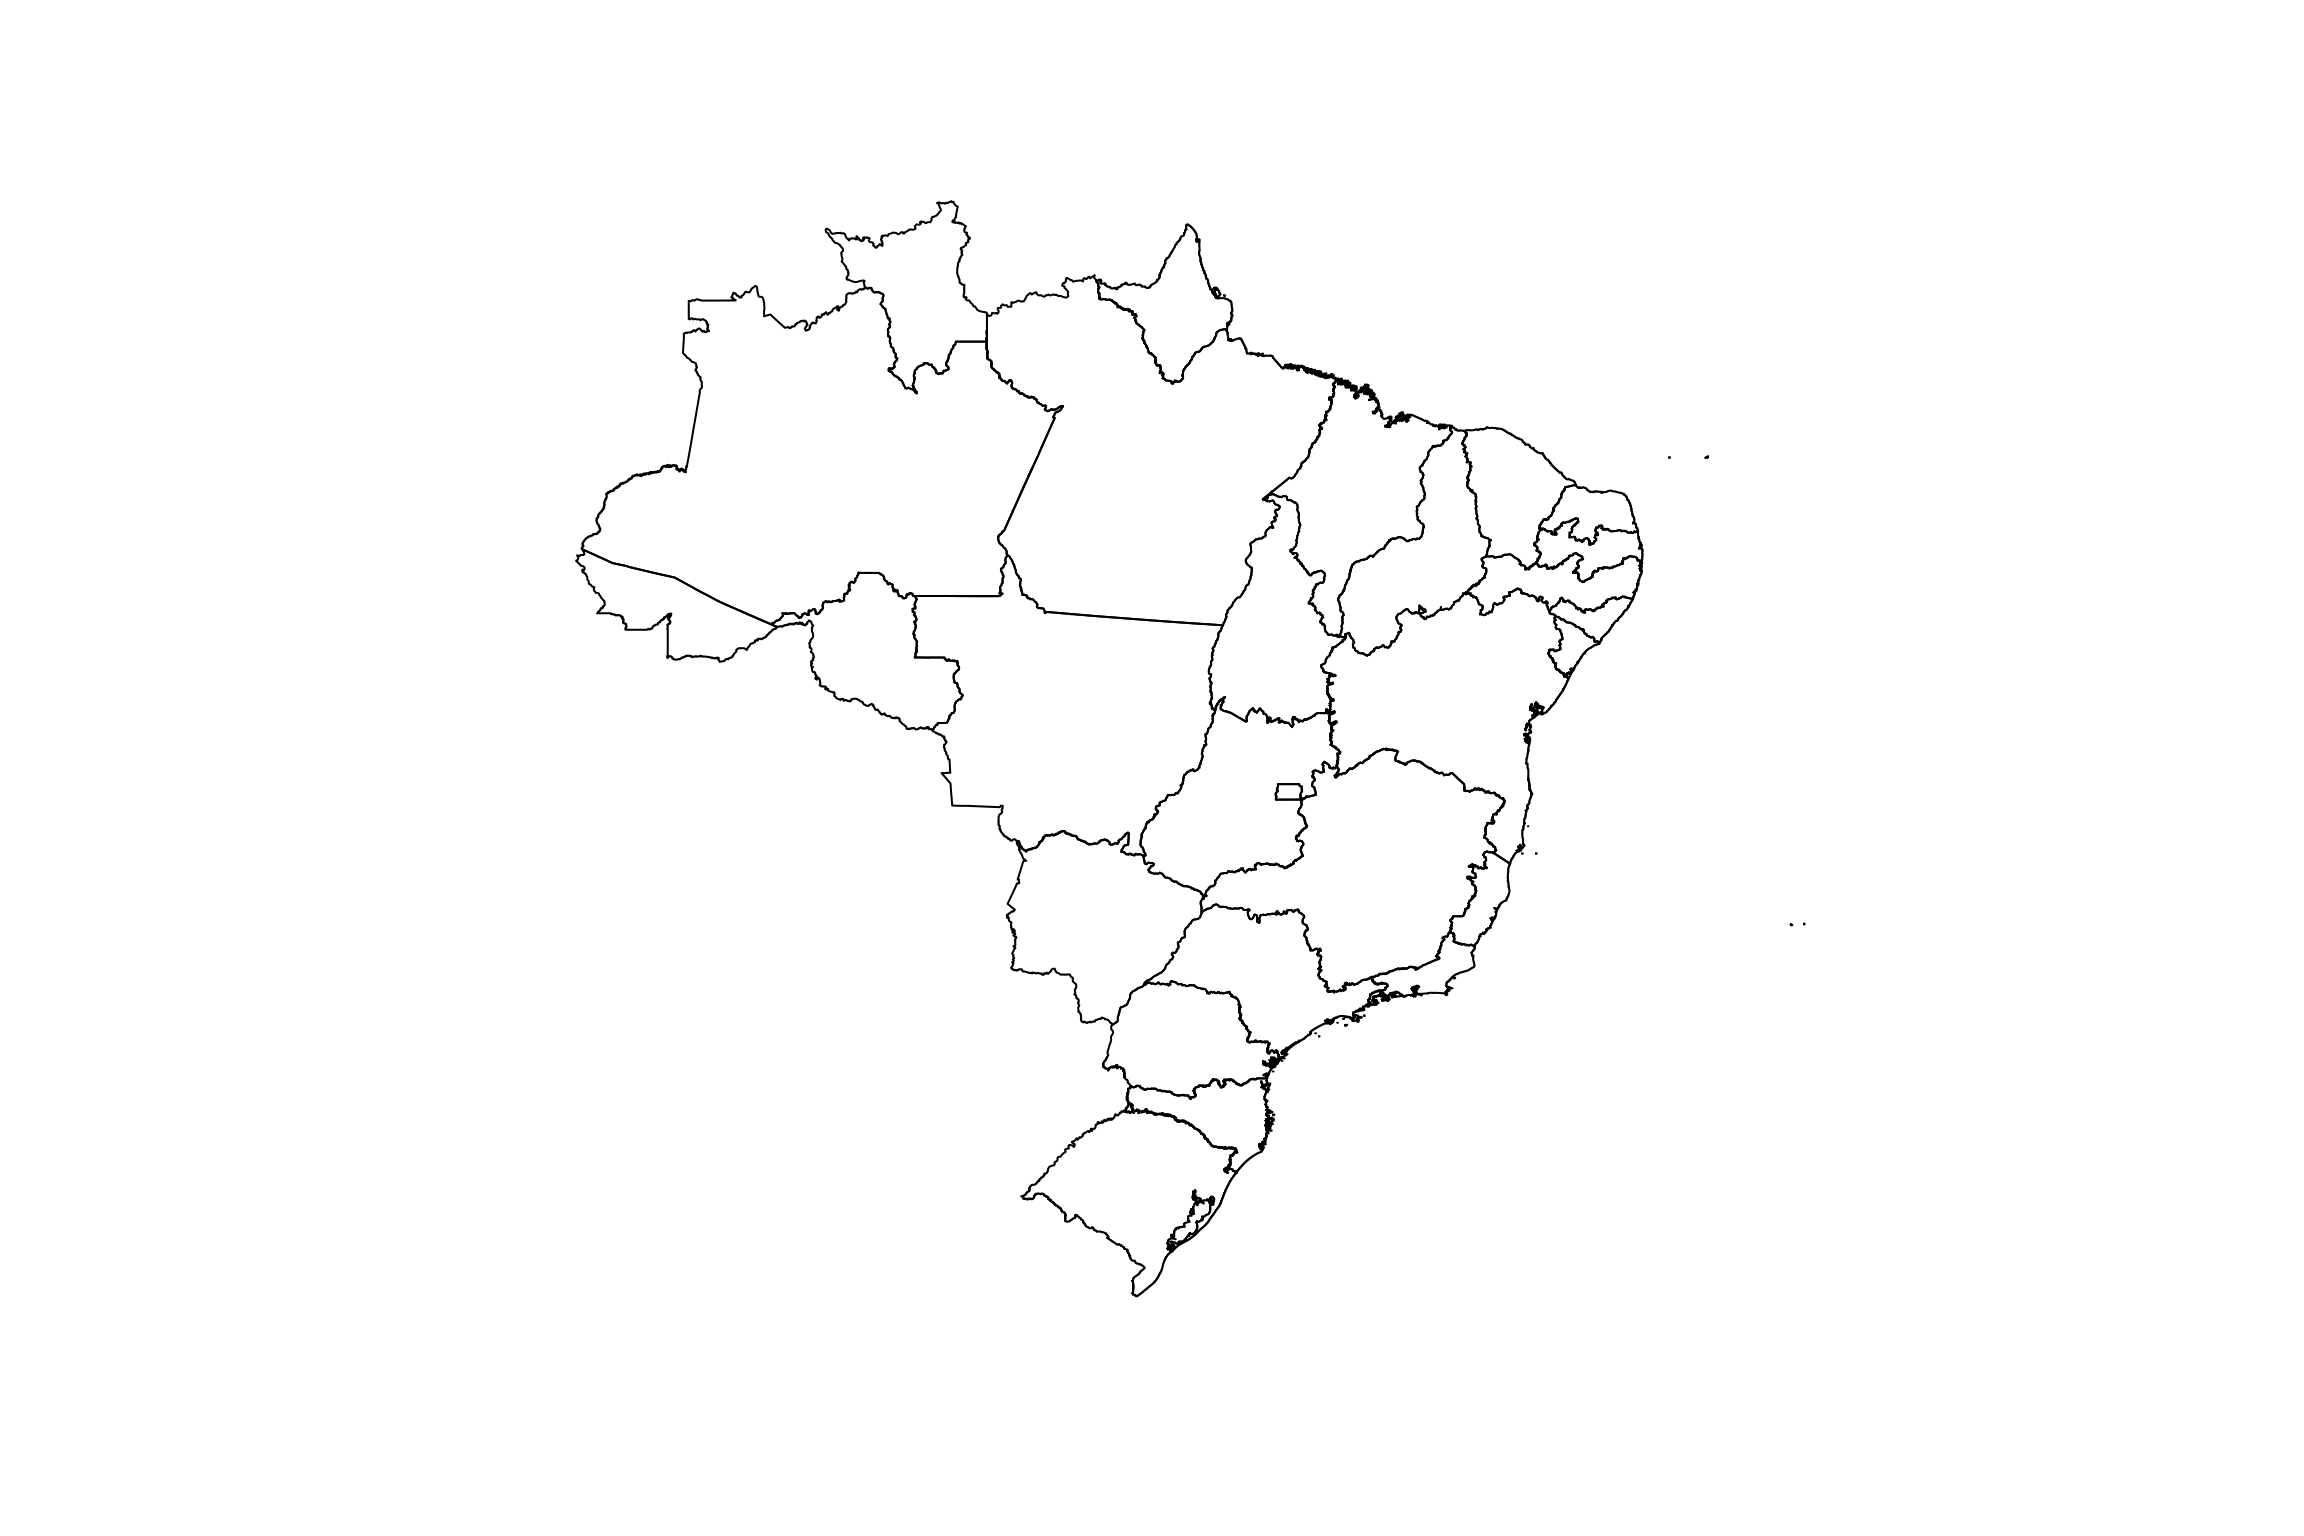
\includegraphics{Trabalho_R_MarkDown_files/figure-latex/unnamed-chunk-21-1.pdf}

\begin{Shaded}
\begin{Highlighting}[]
\KeywordTok{names}\NormalTok{(zones.spwd}\OperatorTok{@}\NormalTok{data)}
\end{Highlighting}
\end{Shaded}

\begin{verbatim}
## [1] "name"   "id.x"   "id.y"   "estado" "cases"  "deaths"
\end{verbatim}

\hypertarget{visualizando-apuxf3s-o-merge}{%
\subsubsection{Visualizando após o
Merge}\label{visualizando-apuxf3s-o-merge}}

\begin{Shaded}
\begin{Highlighting}[]
\KeywordTok{head}\NormalTok{(zones.spwd}\OperatorTok{@}\NormalTok{data, }\DecValTok{10}\NormalTok{)}
\end{Highlighting}
\end{Shaded}

\begin{verbatim}
##                name id.x id.y estado  cases deaths
## 1              Acre   AC   AC     AC  24269    607
## 2           Alagoas   AL   AL     AL  77755   1853
## 3             Amapá   AP   AP     AM 118083   3616
## 4          Amazonas   AM   AM     AP  42285    652
## 5             Bahia   BA   BA     BA 247853   5178
## 6             Ceará   CE   CE     CE 210727   8365
## 7  Distrito Federal   DF   DF     DF 156863   2425
## 8    Espírito Santo   ES   ES     ES 108662   3105
## 9             Goiás   GO   GO     GO 127361   2962
## 10         Maranhão   MA   MA     MA 148923   3402
\end{verbatim}

\hypertarget{visualizando-os-arquivo-zones-gerado}{%
\subsubsection{Visualizando os arquivo Zones
Gerado}\label{visualizando-os-arquivo-zones-gerado}}

\begin{Shaded}
\begin{Highlighting}[]
\NormalTok{zones.spwd}
\end{Highlighting}
\end{Shaded}

\begin{verbatim}
## class       : SpatialPolygonsDataFrame 
## features    : 27 
## extent      : -73.98971, -28.84694, -33.74708, 5.264878  (xmin, xmax, ymin, ymax)
## variables   : 6
## # A tibble: 27 x 6
##    name             id.x  id.y  estado  cases deaths
##    <chr>            <chr> <chr> <chr>   <int>  <int>
##  1 Acre             AC    AC    AC      24269    607
##  2 Alagoas          AL    AL    AL      77755   1853
##  3 Amapá            AP    AP    AM     118083   3616
##  4 Amazonas         AM    AM    AP      42285    652
##  5 Bahia            BA    BA    BA     247853   5178
##  6 Ceará            CE    CE    CE     210727   8365
##  7 Distrito Federal DF    DF    DF     156863   2425
##  8 Espírito Santo   ES    ES    ES     108662   3105
##  9 Goiás            GO    GO    GO     127361   2962
## 10 Maranhão         MA    MA    MA     148923   3402
## # ... with 17 more rows
\end{verbatim}

\hypertarget{manipulando-o-spatial-polyton-gerado}{%
\subsubsection{Manipulando o Spatial Polyton
gerado}\label{manipulando-o-spatial-polyton-gerado}}

\begin{Shaded}
\begin{Highlighting}[]
\KeywordTok{print}\NormalTok{(zones.spwd}\OperatorTok{@}\NormalTok{data}\OperatorTok{$}\NormalTok{cases[[}\DecValTok{1}\NormalTok{]])}
\end{Highlighting}
\end{Shaded}

\begin{verbatim}
## [1] 24269
\end{verbatim}

\begin{Shaded}
\begin{Highlighting}[]
\KeywordTok{print}\NormalTok{(zones.spwd}\OperatorTok{@}\NormalTok{data[[}\DecValTok{1}\NormalTok{,}\DecValTok{1}\NormalTok{]])}
\end{Highlighting}
\end{Shaded}

\begin{verbatim}
## [1] "Acre"
\end{verbatim}

\hypertarget{removendo-acentos-do-spatial-polygon-data-frame}{%
\subsubsection{Removendo acentos do Spatial Polygon DATA
FRAME}\label{removendo-acentos-do-spatial-polygon-data-frame}}

\begin{Shaded}
\begin{Highlighting}[]
\NormalTok{zones.spwd}\OperatorTok{$}\NormalTok{name \textless{}{-}}\StringTok{ }\KeywordTok{remove\_accents}\NormalTok{(zones.spwd}\OperatorTok{$}\NormalTok{name)}
\CommentTok{\#zones.spwd$name.y \textless{}{-} remove\_accents(zones.spwd$name.y)}
\end{Highlighting}
\end{Shaded}

\hypertarget{gerando-o-gruxe1fico-pelo-leaflet-das-regioes-por-geolocation}{%
\subsubsection{Gerando o gráfico pelo LEAFLET das regioes por
GeoLocation}\label{gerando-o-gruxe1fico-pelo-leaflet-das-regioes-por-geolocation}}

\begin{Shaded}
\begin{Highlighting}[]
\NormalTok{bins \textless{}{-}}\StringTok{ }\KeywordTok{c}\NormalTok{(}\DecValTok{0}\NormalTok{, }\DecValTok{50}\NormalTok{, }\DecValTok{75}\NormalTok{, }\DecValTok{100}\NormalTok{, }\DecValTok{150}\NormalTok{, }\OtherTok{Inf}\NormalTok{)}
\NormalTok{pal \textless{}{-}}\StringTok{ }\KeywordTok{colorBin}\NormalTok{(}\StringTok{"YlOrRd"}\NormalTok{, }\DataTypeTok{domain =}\NormalTok{ zones.spwd}\OperatorTok{@}\NormalTok{data[,}\DecValTok{5}\NormalTok{], }\DataTypeTok{bins =}\NormalTok{ bins)}

\NormalTok{state\_popup \textless{}{-}}\StringTok{ }\KeywordTok{paste0}\NormalTok{(}\StringTok{"\textless{}strong\textgreater{}Estado: \textless{}/strong\textgreater{}"}\NormalTok{, }
\NormalTok{                      zones.spwd}\OperatorTok{$}\NormalTok{name.x, }
                      \StringTok{"\textless{}br\textgreater{}\textless{}strong\textgreater{}Casis por 100,000 habitante \textless{}/strong\textgreater{}"}\NormalTok{, }
\NormalTok{                      zones.spwd}\OperatorTok{@}\NormalTok{data[,}\DecValTok{5}\NormalTok{]) }\OperatorTok{\%\textgreater{}\%}\StringTok{ }\KeywordTok{lapply}\NormalTok{(htmltools}\OperatorTok{::}\NormalTok{HTML)}

\KeywordTok{leaflet}\NormalTok{(}\DataTypeTok{data =}\NormalTok{ zones.spwd) }\OperatorTok{\%\textgreater{}\%}
\StringTok{        }\KeywordTok{setView}\NormalTok{(}\DataTypeTok{lng=}\OperatorTok{{-}}\FloatTok{53.2}\NormalTok{, }\DataTypeTok{lat=}\OperatorTok{{-}}\FloatTok{10.33}\NormalTok{, }\DataTypeTok{zoom=}\DecValTok{4}\NormalTok{) }\OperatorTok{\%\textgreater{}\%}
\StringTok{        }\KeywordTok{addProviderTiles}\NormalTok{(}\StringTok{"MapBox"}\NormalTok{, }\DataTypeTok{options =} \KeywordTok{providerTileOptions}\NormalTok{(}\DataTypeTok{id =} \StringTok{"mapbox.light"}\NormalTok{,}
                \DataTypeTok{accessToken =} \KeywordTok{Sys.getenv}\NormalTok{(}\StringTok{\textquotesingle{}MAPBOX\_ACCESS\_TOKEN\textquotesingle{}}\NormalTok{))) }\OperatorTok{\%\textgreater{}\%}
\StringTok{        }\KeywordTok{addPolygons}\NormalTok{(}
                \DataTypeTok{fillColor =} \KeywordTok{topo.colors}\NormalTok{(}\DecValTok{10}\NormalTok{, }\DataTypeTok{alpha =} \OtherTok{NULL}\NormalTok{),}
                \DataTypeTok{weight =} \DecValTok{2}\NormalTok{,}
                \DataTypeTok{opacity =} \DecValTok{1}\NormalTok{,}
                \DataTypeTok{color =} \StringTok{"white"}\NormalTok{,}
                \DataTypeTok{dashArray =} \StringTok{"3"}\NormalTok{,}
                \DataTypeTok{fillOpacity =} \FloatTok{0.7}\NormalTok{,}
                \DataTypeTok{highlight =} \KeywordTok{highlightOptions}\NormalTok{(}
                        \DataTypeTok{weight =} \DecValTok{5}\NormalTok{,}
                        \DataTypeTok{color =} \StringTok{"\#666"}\NormalTok{,}
                        \DataTypeTok{dashArray =} \StringTok{""}\NormalTok{,}
                        \DataTypeTok{fillOpacity =} \FloatTok{0.7}\NormalTok{,}
                        \DataTypeTok{bringToFront =} \OtherTok{TRUE}\NormalTok{),}
                \DataTypeTok{label =}\NormalTok{ pop\_states4,}
                \DataTypeTok{labelOptions =} \KeywordTok{labelOptions}\NormalTok{(}
                        \DataTypeTok{style =} \KeywordTok{list}\NormalTok{(}\StringTok{"font{-}weight"}\NormalTok{ =}\StringTok{ "normal"}\NormalTok{, }\DataTypeTok{padding =} \StringTok{"3px 8px"}\NormalTok{),}
                        \DataTypeTok{textsize =} \StringTok{"15px"}\NormalTok{,}
                        \DataTypeTok{direction =} \StringTok{"auto"}\NormalTok{)) }\OperatorTok{\%\textgreater{}\%}
\StringTok{        }\KeywordTok{addLegend}\NormalTok{(}\DataTypeTok{pal =}\NormalTok{ pal, }\DataTypeTok{values =} \OperatorTok{\textasciitilde{}}\NormalTok{zones.spwd}\OperatorTok{@}\NormalTok{data[,}\DecValTok{5}\NormalTok{], }\DataTypeTok{opacity =} \FloatTok{0.7}\NormalTok{, }\DataTypeTok{title =} \StringTok{"Incidents"}\NormalTok{, }\DataTypeTok{position =} \StringTok{"bottomright"}\NormalTok{)}
\end{Highlighting}
\end{Shaded}

\hypertarget{htmlwidget-db579496360331ca24db}{}
\begin{leaflet}

\end{leaflet}

\hypertarget{lendo-um-arquivo-com-a-populauxe7uxe3o-do-brasil-atuxe9-2019.}{%
\subsubsection{Lendo um arquivo com a população do Brasil até
2019.}\label{lendo-um-arquivo-com-a-populauxe7uxe3o-do-brasil-atuxe9-2019.}}

\begin{Shaded}
\begin{Highlighting}[]
\NormalTok{populacao \textless{}{-}}\StringTok{ }\KeywordTok{read.csv}\NormalTok{(}\StringTok{"\textasciitilde{}/Documents/FIAP/Aula de R/data/populacao.csv"}\NormalTok{, }\DataTypeTok{sep=}\StringTok{";"}\NormalTok{)}
\KeywordTok{head}\NormalTok{(populacao)}
\end{Highlighting}
\end{Shaded}

\begin{verbatim}
##       name populacao  idhm         pib leitos
## 1     Acre    881935 0,719  14.271.000     75
## 2  Alagoas   3337357 0,683  52.843.000    491
## 3    Amapá    845731  0,74  15.480.000     82
## 4 Amazonas   4144597 0,733  93.204.000    502
## 5    Bahia  14873064 0,714 268.661.000   2029
## 6    Ceará   9132078 0,735 147.890.000   1201
\end{verbatim}

\hypertarget{removendo-os-acentos-da-coluna-de-nomes-de-estados}{%
\subsubsection{Removendo os acentos da coluna de nomes de
estados}\label{removendo-os-acentos-da-coluna-de-nomes-de-estados}}

\begin{Shaded}
\begin{Highlighting}[]
\NormalTok{populacao}\OperatorTok{$}\NormalTok{name \textless{}{-}}\StringTok{ }\KeywordTok{remove\_accents}\NormalTok{(populacao}\OperatorTok{$}\NormalTok{name)}
\KeywordTok{head}\NormalTok{(populacao)}
\end{Highlighting}
\end{Shaded}

\begin{verbatim}
##       name populacao  idhm         pib leitos
## 1     Acre    881935 0,719  14.271.000     75
## 2  Alagoas   3337357 0,683  52.843.000    491
## 3    Amapa    845731  0,74  15.480.000     82
## 4 Amazonas   4144597 0,733  93.204.000    502
## 5    Bahia  14873064 0,714 268.661.000   2029
## 6    Ceara   9132078 0,735 147.890.000   1201
\end{verbatim}

\hypertarget{fazendo-o-bind-entre-dois-datasets-e-alterando-o-nome-de-uma-coluna}{%
\subsubsection{Fazendo o BIND entre dois datasets e alterando o nome de
uma
coluna}\label{fazendo-o-bind-entre-dois-datasets-e-alterando-o-nome-de-uma-coluna}}

\hypertarget{utilizando-o-mutate-para-criar-novas-colunas-calculadas}{%
\subsubsection{Utilizando o mutate para criar novas colunas
calculadas}\label{utilizando-o-mutate-para-criar-novas-colunas-calculadas}}

\begin{Shaded}
\begin{Highlighting}[]
\NormalTok{populacao\_bind \textless{}{-}}\StringTok{ }\KeywordTok{cbind}\NormalTok{(populacao, df4)}
\KeywordTok{colnames}\NormalTok{(populacao\_bind)[}\DecValTok{6}\NormalTok{] \textless{}{-}}\StringTok{ "estado"}
\NormalTok{populacao\_bind \textless{}{-}}\StringTok{ }\KeywordTok{mutate}\NormalTok{(populacao\_bind, }\DataTypeTok{casespor100mil  =}\NormalTok{ (populacao\_bind}\OperatorTok{$}\NormalTok{cases }\OperatorTok{/}\StringTok{ }\NormalTok{populacao\_bind}\OperatorTok{$}\NormalTok{populacao)}\OperatorTok{*}\DecValTok{100000}\NormalTok{)}
\NormalTok{populacao\_bind \textless{}{-}}\StringTok{ }\KeywordTok{mutate}\NormalTok{(populacao\_bind, }\DataTypeTok{deathspor100mil  =}\NormalTok{ (populacao\_bind}\OperatorTok{$}\NormalTok{deaths }\OperatorTok{/}\StringTok{ }\NormalTok{populacao\_bind}\OperatorTok{$}\NormalTok{populacao)}\OperatorTok{*}\DecValTok{100000}\NormalTok{)}
\NormalTok{populacao\_bind \textless{}{-}}\StringTok{ }\KeywordTok{mutate}\NormalTok{(populacao\_bind, }\DataTypeTok{letalidade  =} \KeywordTok{round}\NormalTok{(populacao\_bind}\OperatorTok{$}\NormalTok{deaths }\OperatorTok{/}\StringTok{ }\NormalTok{populacao\_bind}\OperatorTok{$}\NormalTok{cases, }\DecValTok{3}\NormalTok{)}\OperatorTok{*}\DecValTok{100}\NormalTok{)}
\KeywordTok{head}\NormalTok{(populacao\_bind)}
\end{Highlighting}
\end{Shaded}

\begin{verbatim}
##       name populacao  idhm         pib leitos estado  cases deaths
## 1     Acre    881935 0,719  14.271.000     75     AC  24269    607
## 2  Alagoas   3337357 0,683  52.843.000    491     AL  77755   1853
## 3    Amapa    845731  0,74  15.480.000     82     AM 118083   3616
## 4 Amazonas   4144597 0,733  93.204.000    502     AP  42285    652
## 5    Bahia  14873064 0,714 268.661.000   2029     BA 247853   5178
## 6    Ceara   9132078 0,735 147.890.000   1201     CE 210727   8365
##   casespor100mil deathspor100mil letalidade
## 1       2751.790        68.82593        2.5
## 2       2329.838        55.52298        2.4
## 3      13962.241       427.55912        3.1
## 4       1020.244        15.73132        1.5
## 5       1666.456        34.81462        2.1
## 6       2307.547        91.60018        4.0
\end{verbatim}

\hypertarget{gruxe1fico-usando-plotly-com-os-nuxfameros-de-casos-por-100-habitantes}{%
\subsubsection{Gráfico usando PLOTLY com os números de casos por 100
habitantes}\label{gruxe1fico-usando-plotly-com-os-nuxfameros-de-casos-por-100-habitantes}}

\begin{Shaded}
\begin{Highlighting}[]
\NormalTok{fig \textless{}{-}}\StringTok{ }\KeywordTok{plot\_ly}\NormalTok{(}
  \DataTypeTok{x =}\NormalTok{ populacao\_bind}\OperatorTok{$}\NormalTok{estado,}
  \DataTypeTok{y =}\NormalTok{ populacao\_bind}\OperatorTok{$}\NormalTok{casespor100mil,}
  \DataTypeTok{name =} \StringTok{"Número de Casos {-} COVID9"}\NormalTok{,}
  \DataTypeTok{type =} \StringTok{"bar"}\NormalTok{,}
  \DataTypeTok{marker =} \KeywordTok{list}\NormalTok{(}\DataTypeTok{color =} \StringTok{\textquotesingle{}rgb(255,140,0)\textquotesingle{}}\NormalTok{)}
\NormalTok{)}

\NormalTok{fig}
\end{Highlighting}
\end{Shaded}

\hypertarget{htmlwidget-f646bf70db21ffc3e817}{}
\begin{plotly}

\end{plotly}

\hypertarget{gruxe1fico-usando-plotly-com-os-nuxfameros-de-mortes-por-100-habitantes}{%
\subsubsection{Gráfico usando PLOTLY com os números de mortes por 100
habitantes}\label{gruxe1fico-usando-plotly-com-os-nuxfameros-de-mortes-por-100-habitantes}}

\begin{Shaded}
\begin{Highlighting}[]
\NormalTok{fig \textless{}{-}}\StringTok{ }\KeywordTok{plot\_ly}\NormalTok{(}
  \DataTypeTok{x =}\NormalTok{ populacao\_bind}\OperatorTok{$}\NormalTok{estado,}
  \DataTypeTok{y =}\NormalTok{ populacao\_bind}\OperatorTok{$}\NormalTok{deathspor100mil,}
  \DataTypeTok{name =} \StringTok{"Número de Casos {-} COVID9"}\NormalTok{,}
  \DataTypeTok{type =} \StringTok{"bar"}\NormalTok{,}
  \DataTypeTok{marker =} \KeywordTok{list}\NormalTok{(}\DataTypeTok{color =} \StringTok{\textquotesingle{}rgb(255,140,0)\textquotesingle{}}\NormalTok{)}
\NormalTok{)}

\NormalTok{fig}
\end{Highlighting}
\end{Shaded}

\hypertarget{htmlwidget-6c7320f4871635fe8b3a}{}
\begin{plotly}

\end{plotly}

\hypertarget{taxa-de-letalidade-por-estado}{%
\subsubsection{Taxa de letalidade por
estado}\label{taxa-de-letalidade-por-estado}}

\begin{Shaded}
\begin{Highlighting}[]
\NormalTok{fig \textless{}{-}}\StringTok{ }\KeywordTok{plot\_ly}\NormalTok{(}
  \DataTypeTok{x =}\NormalTok{ populacao\_bind}\OperatorTok{$}\NormalTok{estado,}
  \DataTypeTok{y =}\NormalTok{ populacao\_bind}\OperatorTok{$}\NormalTok{letalidade,}
  \DataTypeTok{name =} \StringTok{"Número de Casos {-} COVID9"}\NormalTok{,}
  \DataTypeTok{type =} \StringTok{"bar"}\NormalTok{,}
  \DataTypeTok{marker =} \KeywordTok{list}\NormalTok{(}\DataTypeTok{color =} \StringTok{\textquotesingle{}rgb(255,140,0)\textquotesingle{}}\NormalTok{)}
\NormalTok{)}

\NormalTok{fig}
\end{Highlighting}
\end{Shaded}

\hypertarget{htmlwidget-4183f47c3e97352c7e32}{}
\begin{plotly}

\end{plotly}

\hypertarget{agradecimento}{%
\subsubsection{Agradecimento}\label{agradecimento}}

\textbf{Em agradecimento especial ao professor Elthon Freitas do curso
de AI - Turma 14 da FIAP }

Note that the \texttt{echo\ =\ FALSE} parameter was added to the code
chunk to prevent printing of the R code that generated the plot.

\end{document}
